% !TEX root = ../main.tex
\section{实验\chinese{section}}
\subsection{实验题目}
USCI-UART实验
\subsection{实验目的}
上位机(串口调试助手)发指令0xAA,单片机收到指令后发送单字节数据0x55到上位机,采用中断方式,BRCLK=ACLK = REFOCLK = 32768Hz, 波特率9600,LPM3模式。
\subsection{实验仪器和设备}
计算机、开发板、示波器、信号源、电源、Code Composer Studio v5、串口调试助手等。
\subsection{实验步骤}
关闭看门狗,配置串口,设置波特率。打开串口中断和总中断,进入低功耗模式LPM3。当串口接收到数据时,执行中断服务程序,判断数据内容。如果为0xAA,则返回值0x55。
\subsection{程序清单}
\lstinputlisting{src/code/USCIUART1.c}
\clearpage
\subsection{实验结果记录与分析}
\begin{figure}[htbp]
	\centering
	\caption{USCIUART1}
	\label{USCIUART1}
	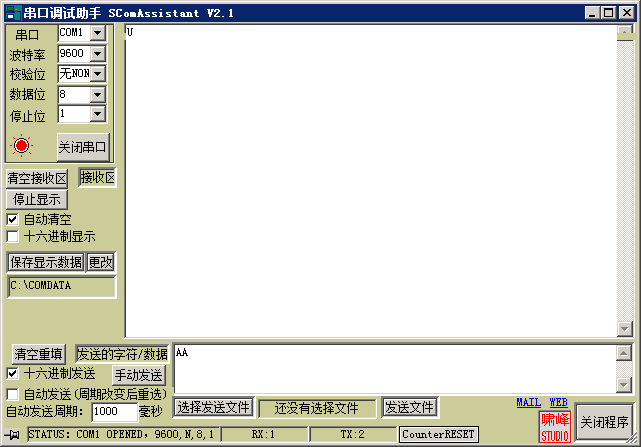
\includegraphics[width=10cm]{bitmap/png/USCIUART1.png}
\end{figure}
\subsection{遇到的问题与解决方法}
\begin{enumerate}
	\item 误以为UB线插入电脑后的COM口就是UART1的COM口。事实上那只是烧程序的COM口而已。
\end{enumerate}
